\documentclass[11pt]{article}
\usepackage[automark]{scrpage2}
\usepackage{lastpage}
\usepackage{pdfpages}
\usepackage[top=3.5cm, bottom=2.5cm, left=2.5cm, right=2.5cm]{geometry}

\pagestyle{scrheadings}
\addtolength{\voffset}{-15pt}
\ihead{Mobile Computing/Alarm-App\\ Gruppe 5 Dokumentation}  
\ohead{Adrian Kurth, Jannes Peters\\ Tjark Kl{\"u}ttermann, Jan Peter Lamp}
\setheadsepline{0.4pt}
\setfootsepline{0.4pt}
\ifoot{Flensburg University of Applied Sciences}  \ofoot{\thepage\space of \pageref{LastPage}}

\begin{document}
	\begin{titlepage}
		\centering
		{\scshape\LARGE Hochschule Flensburg\par}
		\vspace{1cm}
		{\scshape\Large Mobile Computing\par}
		\vspace{1.5cm}
		{\huge\bfseries Alarm-App Dokumentation\par}
		\vspace{2cm}
		{\Large\itshape Adrian Kurth, Jannes Peters, Tjark Kl{\"u}ttermann und Jan Peter Lamp\par}

		
		\vfill
		
		% Bottom of the page
		{\large \today\par}
	\end{titlepage}
\section{Gruppenmitglieder}
\begin{itemize}
	\item Adrian Kurth 590289
	\item Jannes Peters 590252
	\item Tjark Kl{\"u}ttermann 590236
	\item Jan Peter Lamp 590235
\end{itemize}
\section{Aufgabenverteilung}
\begin{itemize}
	\item {\bf UI-Design}\\ Jannes Peters
	\item {\bf Sounddesign}\\ Adrian Kurth und Jannes Peters
	\item {\bf Software-Architektur}\\ Jannes Peters
	\item {\bf Einbinden von OpenCV}\\ Jan Peter Lamp
	\item {\bf Prototyping} \\ Adrian Kurth, Jannes Peters, Tjark Kl{\"u}ttermann und Jan Peter Lamp
	\item {\bf Algorithmus}\\ Adrian Kurth, Jannes Peters, Tjark Kl{\"u}ttermann und Jan Peter Lamp
	\item {\bf Red-Highlighting}\\ Jannes Peters
	\item {\bf Refactoring}\\ Adrian Kurth, Jannes Peters, Tjark Kl{\"u}ttermann und Jan Peter Lamp
\end{itemize}
\section{Programmstruktur}
Das Programm besteht aus einer Activity und einem Custom-View.
\section{Algorithmus}
\includegraphics[scale=0.6]{gleitdings.png}
\begin{center}
	\tiny Die Werte in der Grafik sind Pseudowerte.
\end{center}
Wir messen die Differenz der aufeinanderfolgenden Frames(dunkelblau). Daraus wird ein gleitender Mittelwert errechnet(weinrot). Die Differenz zwischen dem absoluten und dem durchschnittlichen Unterschied wird festgestellt(gr{\"u}n). Davon wird der Durchschnitt berechnet(lila). Der Threshold wird aus wie folgt berechnet:
\[ \mathrm{Gleitender\; Mittelwert\; des\; Bildunterschieds (weinrot)} + (6 * \mathrm{Gleitender\; Mittelwert\; der\; Differenz (lila)}) \]
wobei die 6 ein durch Testen herausgefundener Faktor ist.\\
Die {\"A}nderung der Bilder wird durch eine Matrize dargestellt. Um die aktuelle {\"A}nderung in den Frame einzuzeichnen, wird die aktuelle {\"A}nderung in den roten Kanal eines leeren Bildes kopiert. Dieses Bild wird dann mit dem Schwarz-Wei\ss-Bild addiert und gezeichnet. Somit sieht man die {\"A}nderungen in rot auf dem Bild.
\section{Klassen}
\subsection{MainActivity.java}
Die MainActivity ist die View und der Controller. Hier befindet sich die State-Machine der App.
\subsection{AlarmCameraView.java}
Diese Klasse erweitert die JavaCameraView von OpenCV um die Funktionalit{\"a}t des Alarms.
\section{Materialien}
\begin{itemize}
	\item Android Studio 3
	\item Asus Zenfone 2 (Android CM 7.1.2)
	\item OnePlus X (Android 6.0.1)
	\item Asus Zenfone 2 (Android 5.0)
	\item Discord (Voicechat)
	\item Teamviewer 13
	\item Git
\end{itemize}
\section{Testbericht}
Die App wurde verschiedenen Smartphones und Android-Versionen getestet (siehe Punkt Materialien). Dabei lief die App problemlos auf allen Ger{\"a}ten. \\
Um zu Pr{\"u}fen, ob die App zum richtigen Zeitpunkt ausl{\"o}st, haben wir verschiedene Bewegungen und Schattenbilder getestet.
\section{Probleme}
Folgende Probleme traten w{\"a}hrend der Entwicklung auf:
\begin{itemize}
	\item {\bf Android Dokumentation f{\"u}r OpenCV nicht vorhanden}\\ Dadurch war es manchmal schwierig, den Ort von Funktionen oder Konstanten zu finden, selbst wenn man sie in der C-Dokumentation gefunden hat.
	\item {\bf Nur OpenCV-Version 2.4.2 lief ohne Probleme}\\ Alle anderen Versionen liefen nur teilweise oder gar nicht(SIGSEV-Fehler bei einigen Funktionen).
	\item {\bf Renderfehler}\\ Dies ist ein nicht reproduzierbarer Fehler, der manchmal auftritt und durch einen Neustart behebbar ist.\\
	\begin{center}
		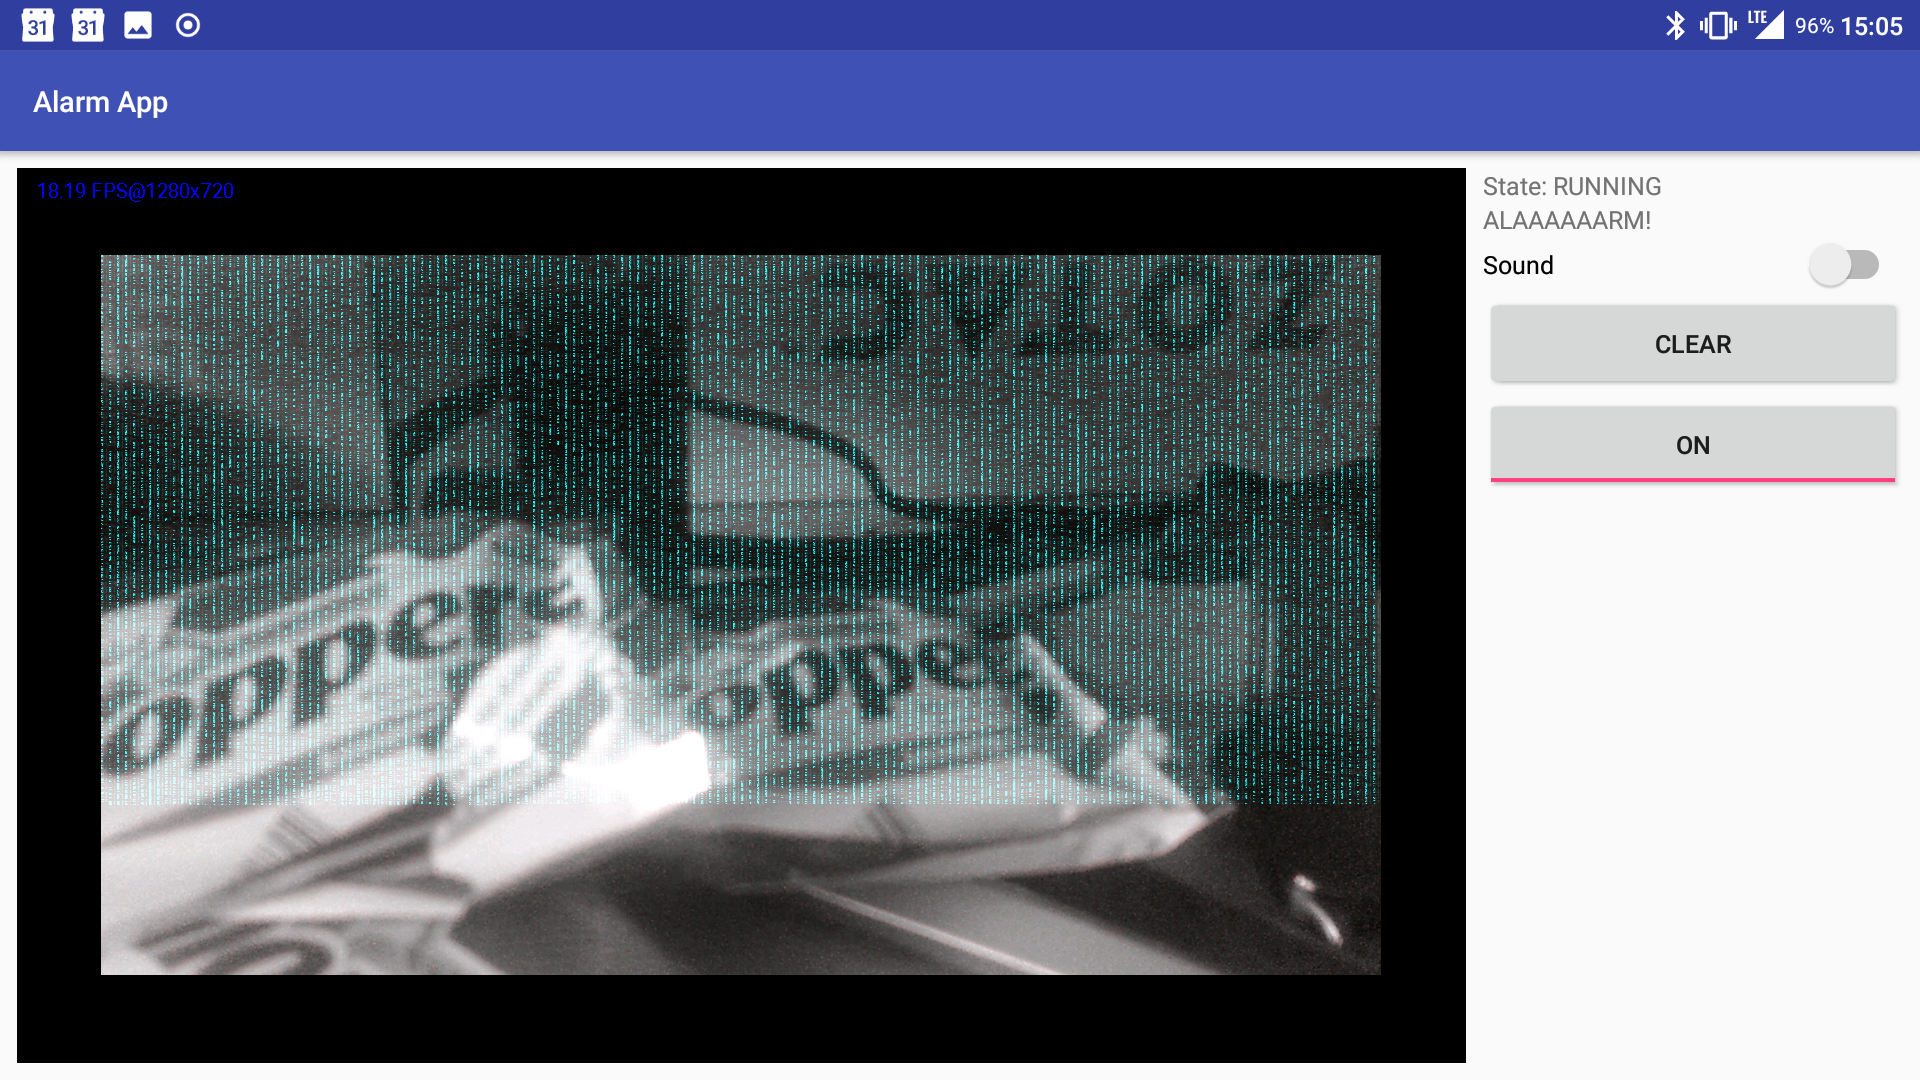
\includegraphics[scale=0.2]{bug-jannes.png}
	\end{center}
\end{itemize}
\section{Sourcen}
\subsection{MainActivity.java}
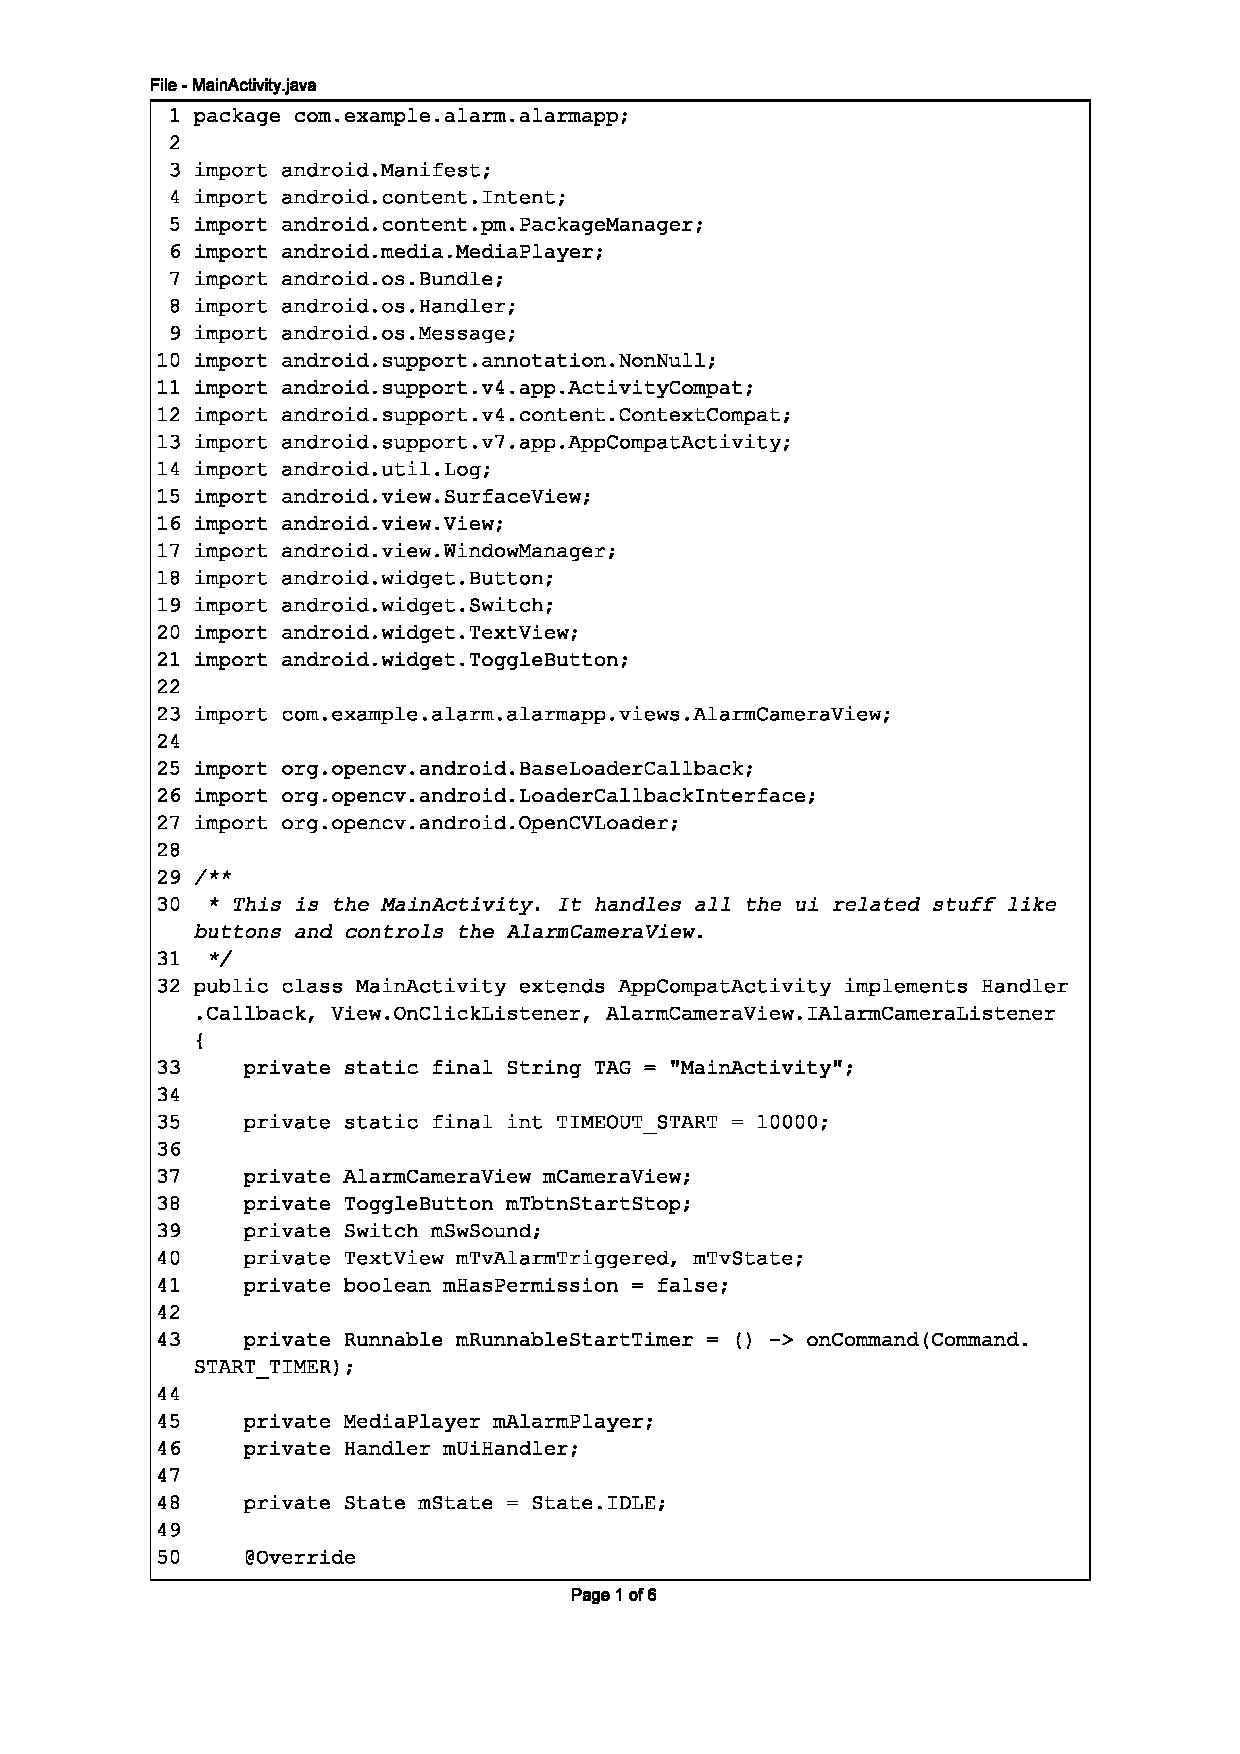
\includegraphics[scale=0.75]{MainActivity.pdf}
\includepdf[pages=2-, scale=0.75, pagecommand={\pagestyle{scrheadings}}]{MainActivity.pdf}
\subsection{AlarmCameraView.java}
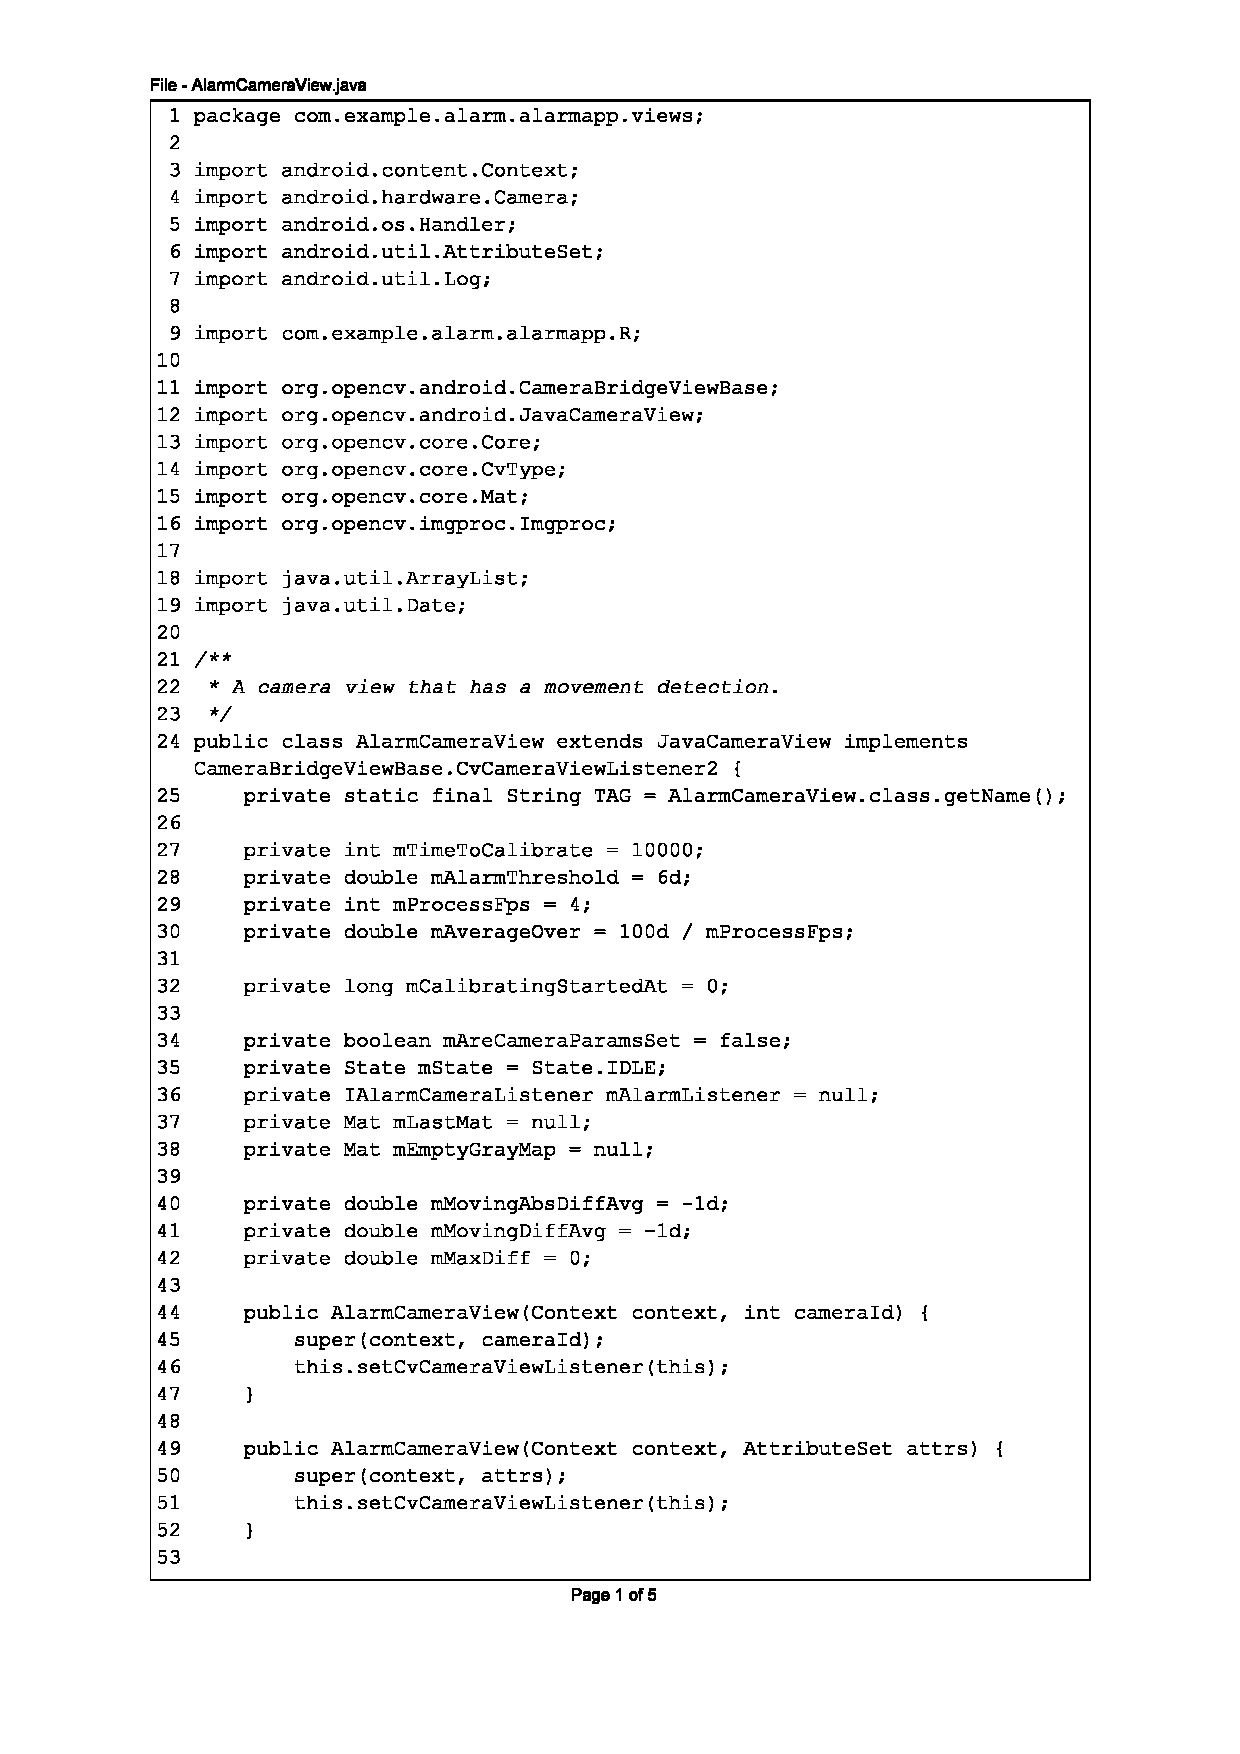
\includegraphics[scale=0.75]{AlarmCameraView.pdf}
\includepdf[pages=2-, scale=0.75, pagecommand={\pagestyle{scrheadings}}]{AlarmCameraView.pdf}
\subsection{AndroidManifest.xml}
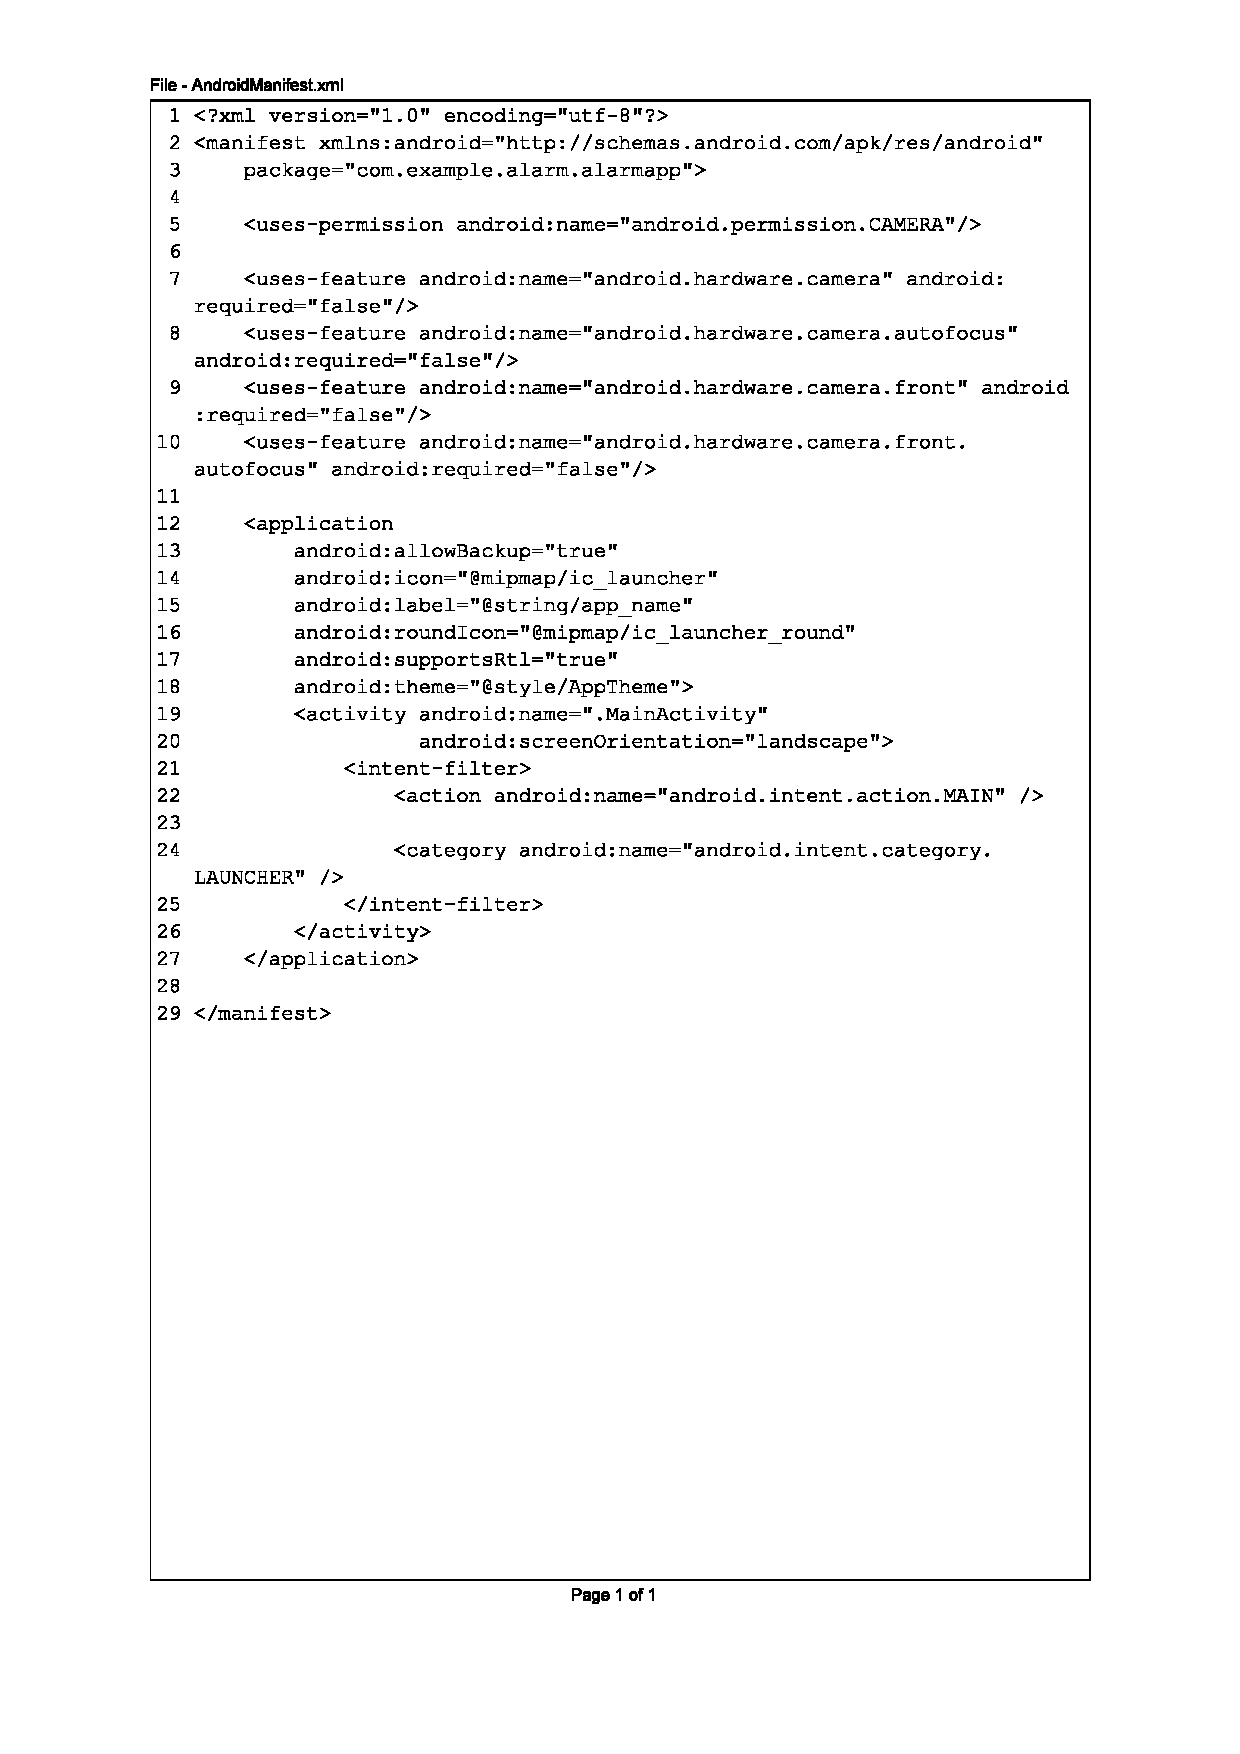
\includegraphics[scale=0.75]{AndroidManifest.pdf}
\subsection{activity\_main.xml}
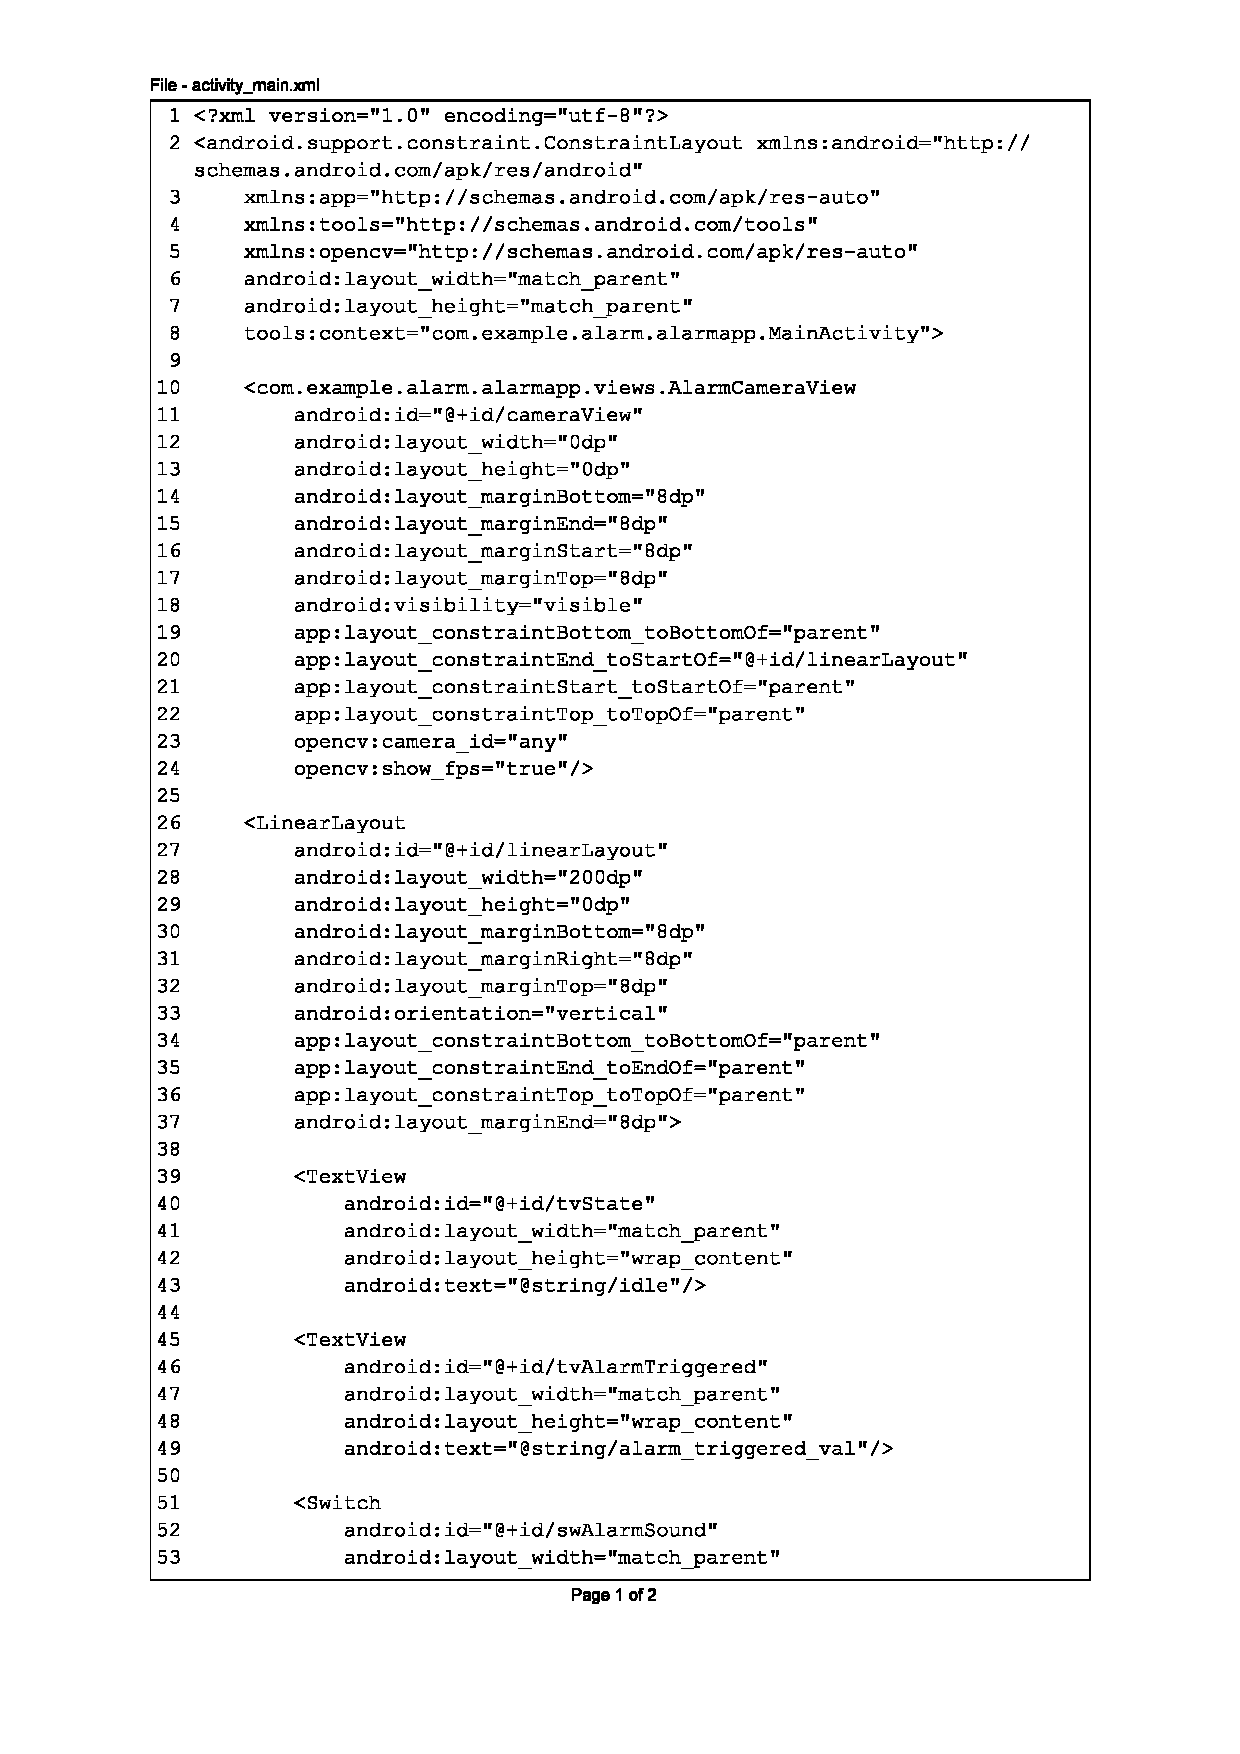
\includegraphics[scale=0.75]{activity_main.pdf}
\includepdf[pages=2-, scale=0.75, pagecommand={\pagestyle{scrheadings}}]{activity_main.pdf}
\subsection{activity\_main\_permission\_missing.xml}
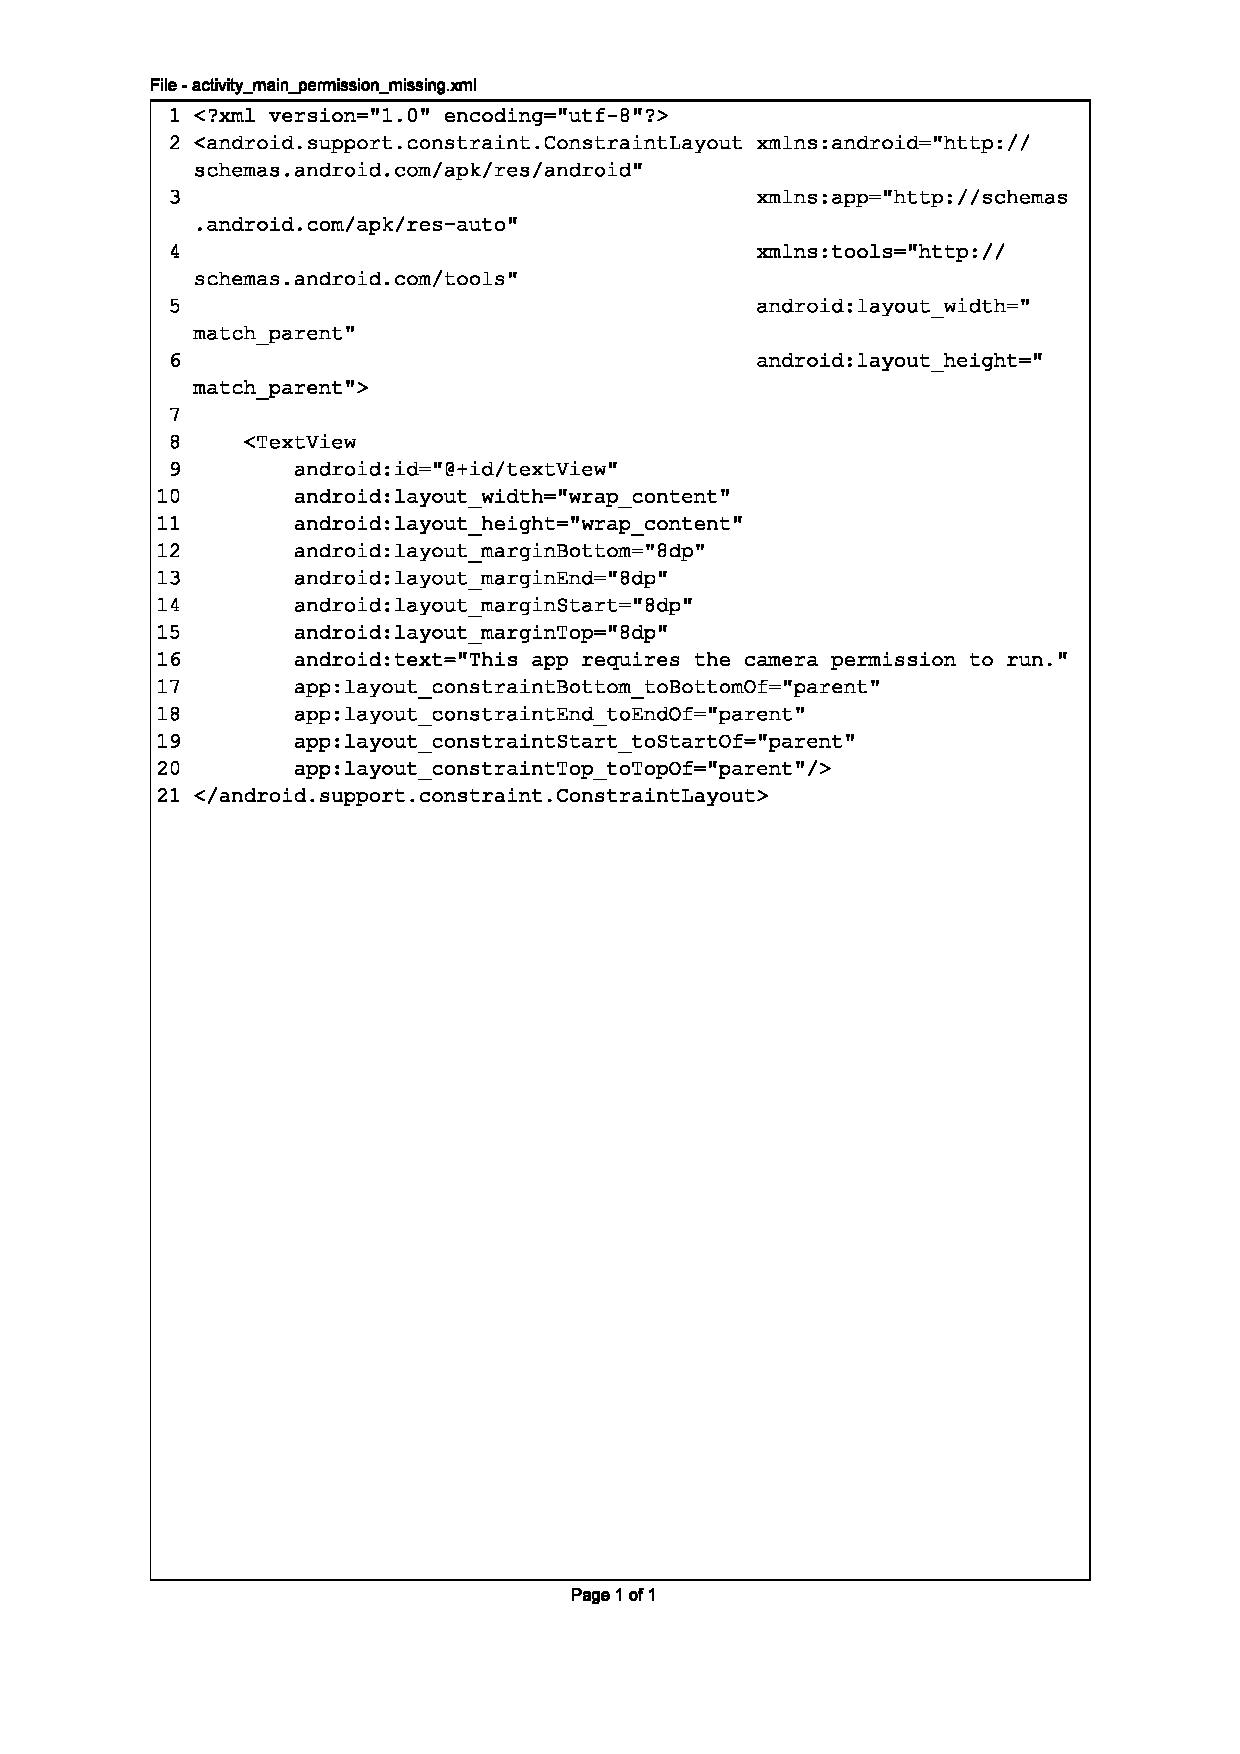
\includegraphics[scale=0.75]{activity_main_permission_missing.pdf}
\end{document}